\pdfbookmark[1]{Background_introduction}{background_introduction}
% \chapter{Background - The building blocks of superconducting qubits}\label{chap:background_introduction}
\begin{figure}[h]
    \centering
        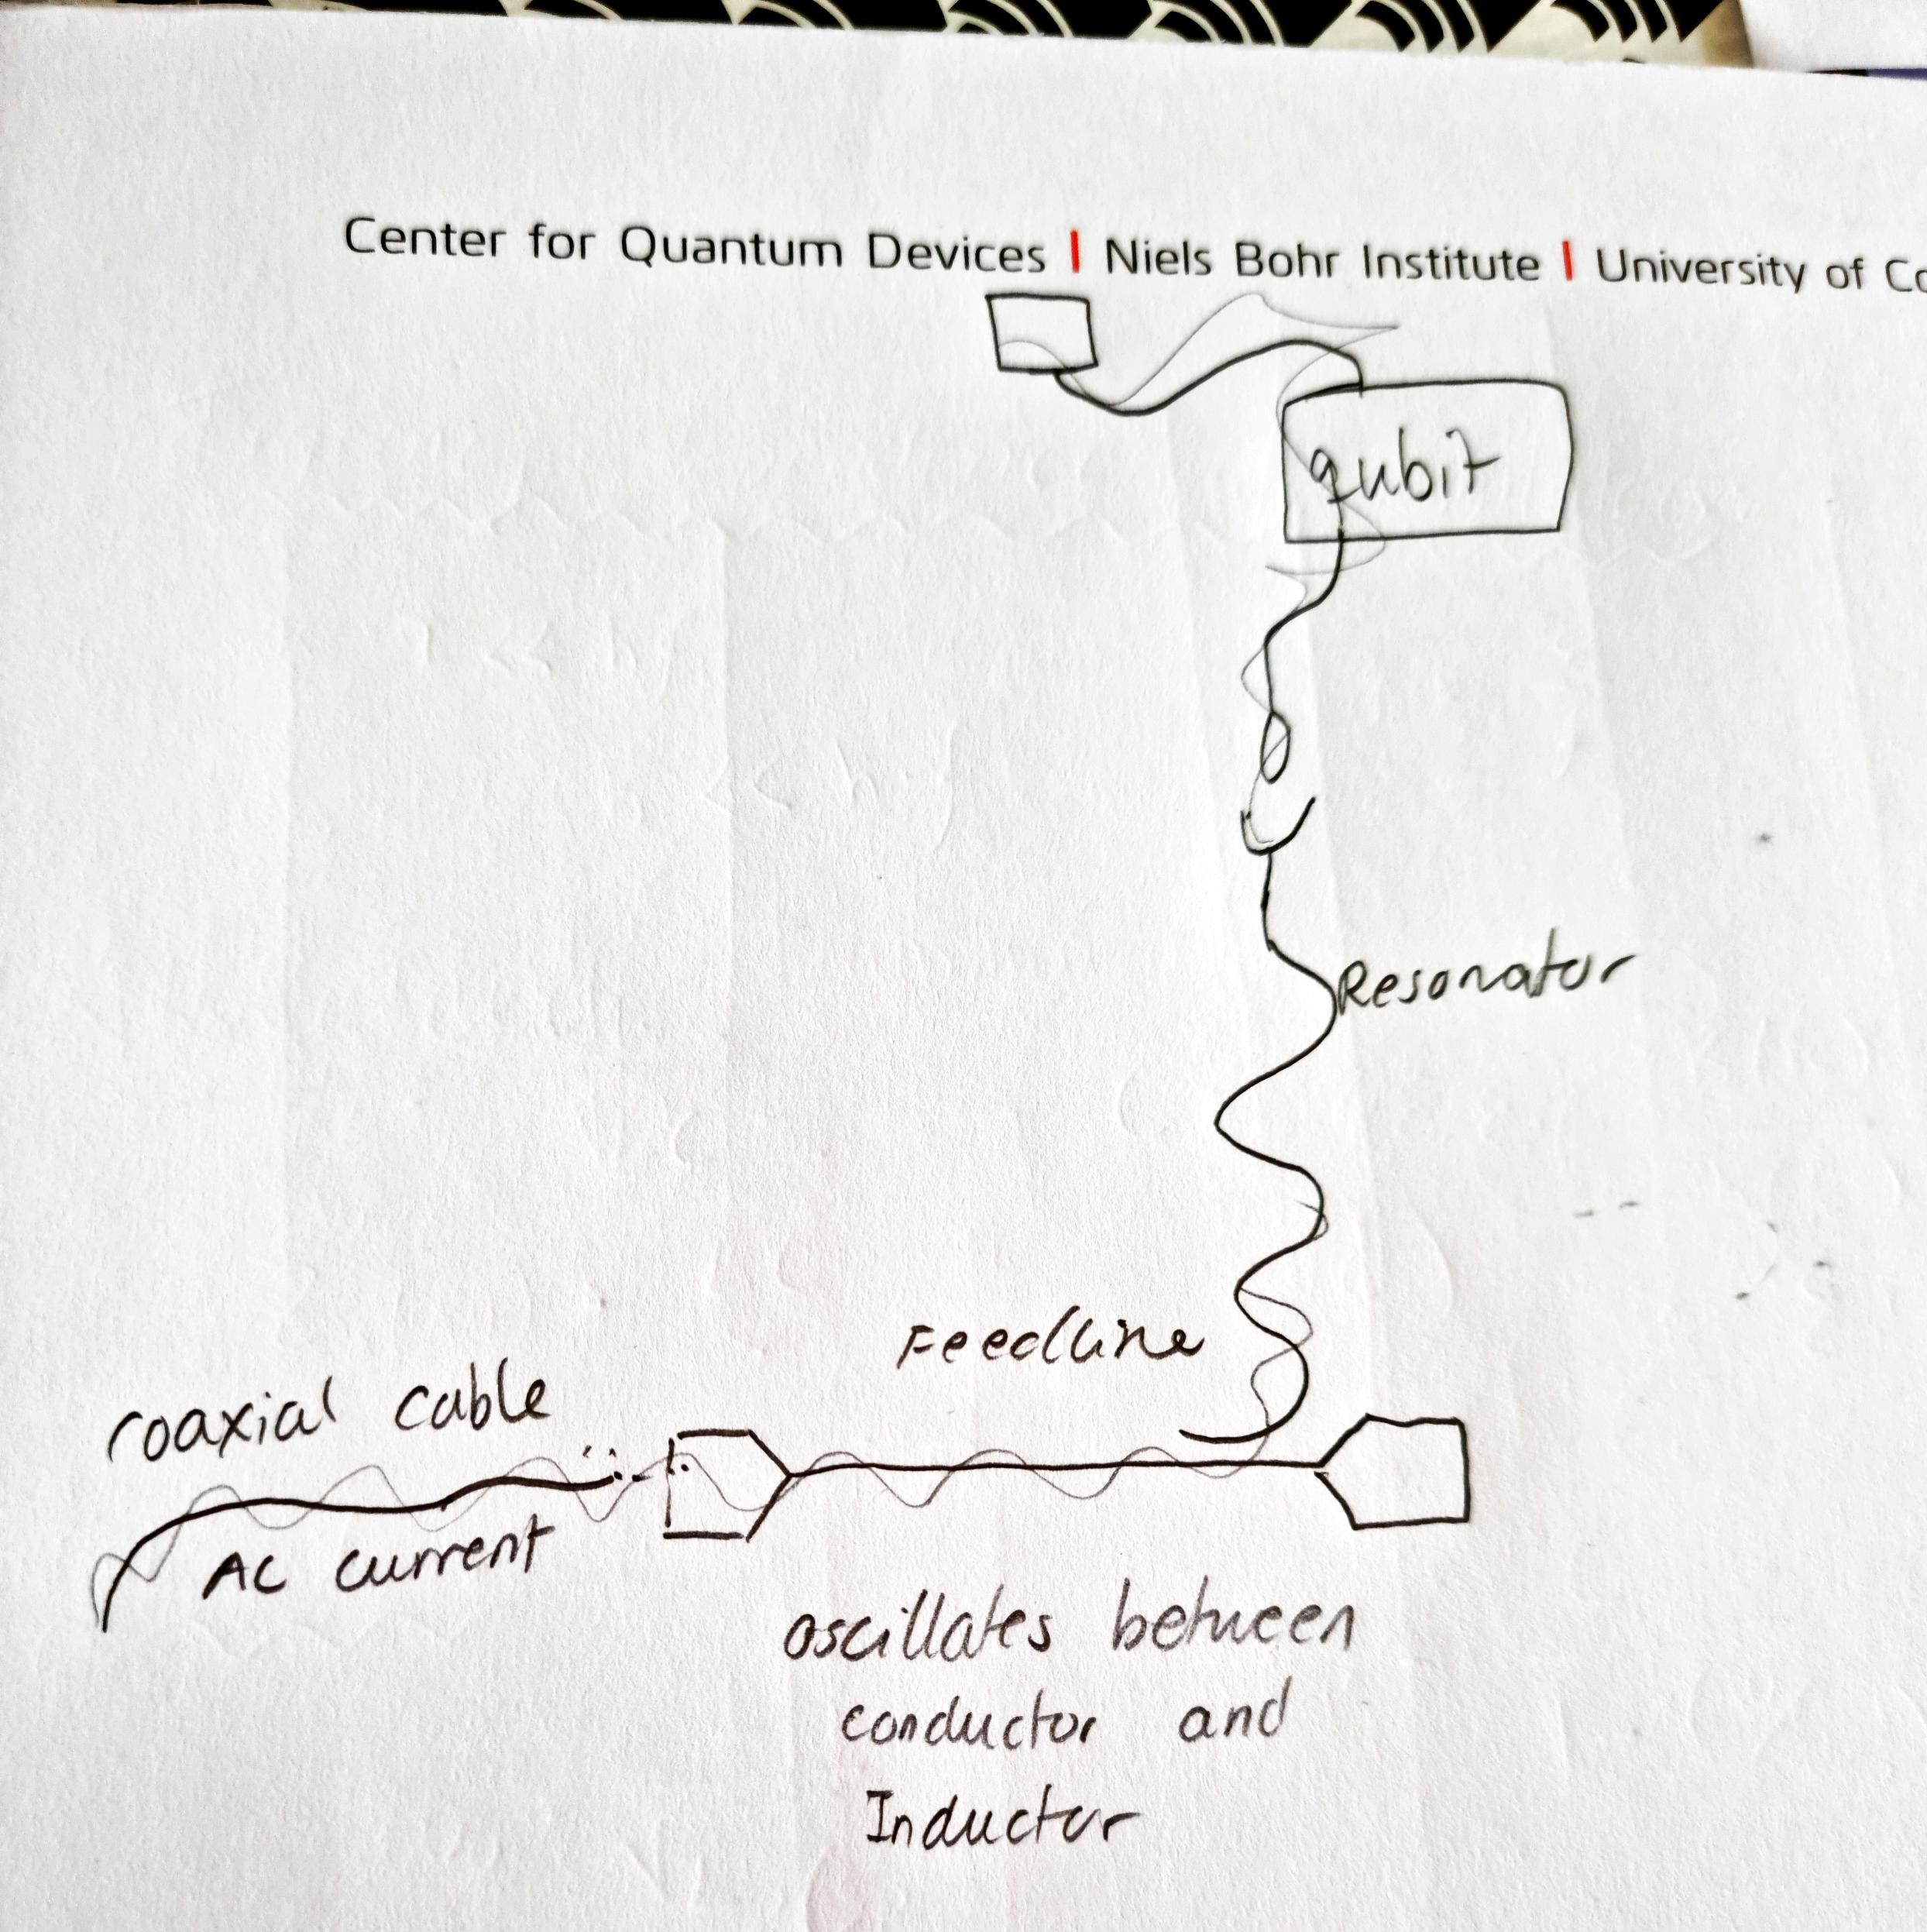
\includegraphics[width = 13cm]{Images/picture_of_setup_qpu copy.png}
        \caption[Chip overview]{\textbf{Chip overview:} This is an overview of the whole chip with the feedline, resonators and the qubits from a top view (A) and from the side view (B).}
        \label{fig:setup_qpu}
\end{figure}
%  The setup
A quantum processing unit, \acrshort{qpu}, is the heart of any quantum computer technology just like the central processing unit, \acrshort{cpu}, is of a classical computer. The fundamental building blocks of superconducting QPU design consists of superconducting transmission lines, coplanar waveguide resonators, and Josephson junctions. These components, interconnected with precision, form the cornerstone of quantum circuits that can be combined in tons of different ways to build a \acrshort{qpu} using superconducting circuits. The fig. \ref{fig:setup_qpu} is the picture of what a general model of a \acrshort{qpu} utilizing fluxonium, superconducting qubit, looks like. The coaxial cables are connected to a transmission which is capacitively coupled to a resonator connected to the qubit. The qubit is also connected to a source (typically a direct current, \acrshort{dc}, source) (called the drive line?). Each component in the circuit and each intersection between the components are described by a lot of different physics. This section aim to build a foundation for understanding some of the physics behind a fluxonium circuit. Superconducting circuits for quantum computing is a very big field utilizing many different aspects of physics, chemistry and computer science however we only briefly glance upon a few out of many interesting subareas.  
\\
% The different components we need to understand
The physics we need to take into account already start with the standard coaxial cable as the impedance needs to be matched throughout the system for eliminating reflections and power loss \cite{Pozar2012}. These happens in the interface between the coaxial cable and the feedline or the feedline and the resonator. For this we need to understand how the electromagnetic waves behave in different media and with different boundary conditions as well as how to calculate the right physical properties. It's also essential to know what types of losses can be and how we can avoid them. This field of physics is often called waveguide quantum electrodynamics. 
\\
As we are working with superconducting circuits, we also is interested in how superconductivity is obtained in different materials and what criteria for the surroundings should be present for getting the optimal environment for our qubits. 
\\
It is crucial to understand some aspects of electrical engineering and how the different components work not only from a physics perspective, but also what the role of the different components are in a circuitry. Of course we also need the knowledge we have from condensed matter physics to describe the non-linear Josephson element which are the key element for all superconducting qubits circuits.
\\
People often associate cavity QED in quantum optics with the model for the qubit in the system seen in fig.???. In this comparison, the resonators carries only the specific engineered frequencies (not sure this is why) and can be thought of as the cavity. The qubit is the 2 level system and the electromagnetic wave guided trough the system is the wave. Therefore we also take a short look into the quantum optics to describe the interaction between our 2 level system qubit and the microwave which controls it.
\\
% What is discussed in this section
In the background section we go through the theory for making the resonators, then the JJ, then the array of JJ and we talk about how to put these components together to form superconducting qubits mentioning the physics behind superconducting qubits heroff the transmon qubits, flux qubits and fluxonium. We end the chapter by discussing different advantages in the Fluxonium community up to now (this will also serve as an introduction to the simulation part.)
